\chapter{Entorno virtual}

% **************************** Define Graphics Path **************************
\graphicspath{{Chapter3/Figs/}}

Uno de los principales objetivos de este trabajo es realizar pruebas funcionales y de escala sobre la arquitectura del prototipo. Es de interés generar distintas realidades, y así detectar puntos de falla o variables clave en la performance de la arquitectura. Para esto se puede utilizar dos parámetros: topología y servicios. Es importante poder aplicar topologias complejas y relativamente grandes a la arquitectura, así como grandes cantidades de servicios, y de esta forma encontrar posibles problemas con la arquitectura, y su respectiva solución. Dado que no es realista hacer este tipo de pruebas con un prototipo físico, por temas económicos y prácticos, se observa la necesidad de un entorno virtual capaz de simular las características del prototipo. En este capítulo se estudian los requerimientos que debe cumplir este entorno, las herramientas estudiadas para lograrlo, y los detalles de diseño e implementación de la solución construida.

\section{Requerimientos del entorno virtual}
Los requerimientos de este entorno se pueden dividir en dos grupos. En primer lugar, la idea es que el entorno virtual se comporte de una forma lo más fiel posible al prototipo físico. Esto no quiere decir que deba usar las mismas herramientas, pero es deseable que así sea. En segundo lugar, hay que considerar los requerimientos inherentes de un entorno de simulación como el que se pretende. El primer grupo se detalla a continuación.

\begin{itemize}
	\item Se debe poder simular múltiples RAUSwitch virtuales, y los mismos deben tener las mismas capacidades funcionales que sus pares físicos. A partir de esto, se desprenden los siguientes sub-requerimientos.
	\begin{itemize}
		\item Deben poder ejecutar el protocolo de enrutamiento OSPF. Es deseable que lo hagan mediante la suite de ruteo Quagga.
		\item Deben soportar el protocolo OpenFlow 1.3. Esto se debe a que la aplicación que implementa VPNs depende de que los switches tengan soporte para MPLS, y OpenFlow ofrece esta funcionalidad a partir de la versión 1.3 (???). Es muy deseable que lo hagan mediante OpenVSwitch, ya que es lo que utilizan los RAUSwitch físicos.
	\end{itemize}
	\item Se debe poder simular múltiples hosts, ya que son los agentes que se conectan a la red y se envían tráfico entre sí, para corroborar que los flujos de datos son correctos.
	\item La aplicación RAUFlow debe ejecutarse y comunicarse correctamente con los RAUSwitch. Esto implica que el controlador Ryu debe ser soportado por el entorno.
\end{itemize}

Cabe remarcar que los módulos SNMP y LSDB Sync quedan por fuera de los requerimientos principales, por ser no esenciales. \\

El segundo grupo de requerimientos es más genérico, ya que son los que surgen para casi cualquier entorno de simulación de redes.

\begin{itemize} 
	\item Facilidad de configuración. Es importante que el entorno pueda generar distintas topologias y escenarios sin demasiado esfuerzo de configuración.
	\item Escalabilidad. Dado que uno de los objetivos es realizar pruebas de escala, el entorno debería ofrecer buena escalabilidad en la cantidad de nodos que puede simular. Esto se traduce a que una computadora promedio de uso personal pueda levantar algunas decenas de nodos virtuales como mínimo.
\end{itemize}

\section{¿Por qué Mininet?}


\section{Diseño e implementación del entorno}
El entorno está construido alrededor de Mininet, y se podría pensar como una extensión de la misma. \textit{Out of the box}, Mininet ya cumple la mayoría de los requerimientos estudiados anteriormente. Está diseñada para ser escalable, ya que usa containers reducidos, tiene soporte para OpenFlow 1.3 mediante OpenVSwitch, y gracias a su API en Python es muy fácil de configurar. El aspecto en el que falla es en el soporte para Quagga. Dado que Mininet es una herramienta de prototipado para SDN puro, no está pensado para un esquema híbrido como el que se propone. Los switches compatibles con OpenVSwitch que ofrece no pueden tener su propio network namespace, por lo tanto, no pueden tener su propia tabla de ruteo ni interfaces de red aisladas, así que no es posible que utilicen Quagga.

Por otro lado, los hosts de Mininet sí tienen su propio network namespace, y gracias a su capacidad de tener sus propios procesos y directorios, podemos ejecutar una instancia de Quagga y OpenVSwitch para cada host. De esta forma es posible crear un router como el requerido por la arquitectura. Esta extensión de las funcionalidades de los hosts es posible ya que Mininet está programado con orientación a objetos y permite al usuario crear subclases propias de las clases que vienen por defecto. En la figura \ref{fig:clases_entorno} se puede ver la estructura de clases del entorno construido. En las siguientes secciones se procederá a estudiar cada una de ellas.

\begin{figure}[t]
	\caption{Diagrama de clases del entorno.}
	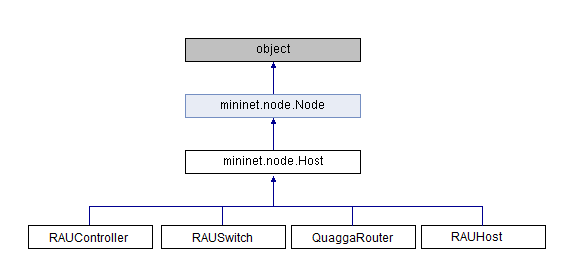
\includegraphics[scale=0.65]{clases_entorno}
	\centering
	\label{fig:clases_entorno}
\end{figure}

\subsection{RAUController}
En el uso típico de Mininet, la comunicación entre el controlador y el switch se da a través de la interfaz de loopback. Esto es así porque los switches no tienen su propio namespace. Para lograr dicha comunicación, no hace falta un objeto en Mininet que represente el controlador, ya que ejecutar la aplicación en el sistema operativo base ya habilita al switch a comunicarse con ella a través de la interfaz de loopback. Esta situación cambia en este diseño, porque los switches pasan a tener su propio network namespace. Esto lleva a la necesidad de crear un host virtual, que ejecute la aplicación de RAUFlow y se comunique con los switches a través de enlaces virtuales. Para satisfacer esta necesidad se usa la clase RAUController.

\subsection{RAUSwitch}
La clase RAUSwitch es el núcleo del entorno de simulación. Es un Host extendido de tal forma para que, gracias a la funcionalidad de directorios privados, ejecute su propia instancia de Quagga y OpenVSwitch. Cada RAUSwitch tiene los siguientes directorios privados: /var/log/, /var/log/quagga, /var/run, /var/run/quagga, /var/run/openvswitch. Cada RAUSwitch también usa un directorio bajo /tmp, para almacenar sus archivos de configuración.\\ \\

OpenVSwitch básicamente consiste de 2 demonios (ovs-vswitchd y ovsdb-server) que ejecutan en el user-space, y un módulo en el kernel que actúa como cache para los flujos recientes. Utiliza el protocolo 'netlink' para comunicar el user-space con el módulo en el kernel. Poder tomar decisiones sobre los paquetes a nivel del kernel, sin tener que pasar por el user-space, explica en gran medida el buen nivel de performance que ofrece OpenVSwitch. Sin embargo, tener múltiples módulos de kernel ejecutando en el mismo sistema operativo puede crear comportamientos impredecibles e incorrectos, ya que no está previsto para trabajar de esa forma.\\
Afortunadamente, OpenVSwitch puede ejecutarse completamente en modo user-space, es decir, sin soporte del módulo del kernel. Esto implica que podemos ejecutar tantas instancias de OpenVSwitch como queramos, pero la performance va a ser significativamente peor. Esto no es una desventaja muy seria, ya que el objetivo del entorno no es ser performante al procesar paquetes. Cabe aclarar que en este modo OpenVSwitch continúa haciendo cacheo de flujos, pero ahora lo hace en el user-space.

\begin{figure}[t]
	\caption{Arquitectura de OpenVSwitch.}
	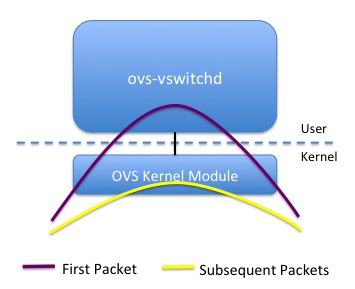
\includegraphics[scale=0.65]{ovs_dataplane}
	\centering
	\label{fig:ovs_dataplane}
\end{figure}

\subsection{QuaggaRouter}
Es una clase similar al RAUSwitch pero sin OpenVSwitch, es decir, sólo usa Quagga. Apunta a representar el router CE que utilizaría una subred para conectarse a la red. Está conectado a un RAUSwitch de borde.

\subsection{RAUHost}
Representa a los hosts que serán clientes de la red. Con este propósito, se podría utilizar directamente la clase Host de Mininet, pero se construye esta clase auxiliar para evitar determinadas configuraciones manuales, como por ejemplo, el \textit{default gateway}.

\subsection{LSDB Sync}
Explicar que se cambió SNMP por OVS

\section{Modo de uso del entorno}
En Mininet estándar, las topologias se crean mediante la API en Python. Se crea un objeto de tipo Topology, se le agregan los nodos que se desee, y se establecen los enlaces virtuales entre esos nodos. Como el entorno es en esencia una extensión de Mininet, hereda su facilidad de uso. La única diferencia radica en que las entidades de este entorno requieren parámetros adicionales para su creación, que serán detallados en el Anexo.

\subsection{GraphML Loader}

\section{Problemas y errores encontrados}
Como resultado de las pruebas funcionales básicas que se efectuaron sobre el entorno (que son detalladas en la sección 4.1.1) se detectaron determinados problemas que fueron necesarios estudiar. Esta sección explicará en que consiste cada problema, estudiando sus síntomas, su explicación, y en caso de que exista una, su solución. Como se verá, algunos de ellos se manifestarían en un despliegue real de la arquitectura, y otros son a causa del uso de un entorno virtual, y por lo tanto no se deberían tener en cuenta en un despliegue real.

\subsection{Errores en el código de RAUFlow}
Se descubrió que existían determinados errores (o "bugs") en el código de RAUFlow. Como son errores en el código del controlador, es importante remarcar que estos errores sin lugar a dudas se manifestarían en una red real. \\ \\
\textbf{Error en flujos de servicio con más de un salto} \\
\begin{figure}[t]
	\caption{Escenario donde los flujos están mal configurados. Muestra la topología de la red y los flujos de interés para cada nodo.}
	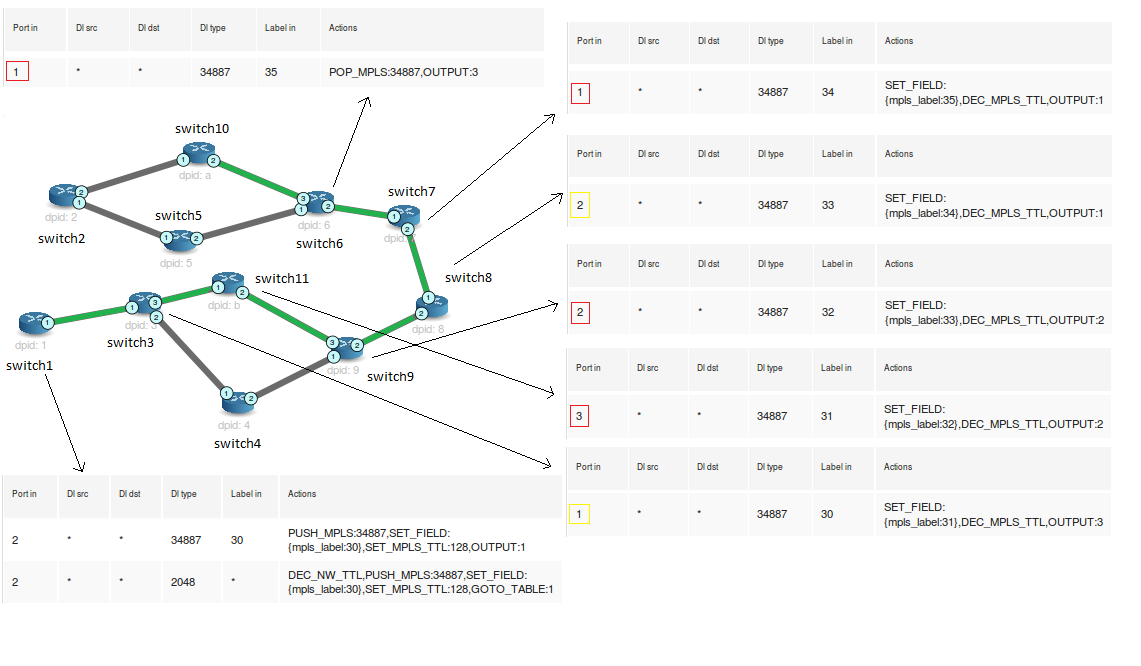
\includegraphics[scale=0.5]{flujos_incorrectos}
	\centering
	\label{fig:flujos_incorrectos}
\end{figure}
Se observó que cuando se trataba de crear un servicio que pasara por más de 2 nodos (es decir, con más de un salto), el controlador instalaba flujos en los nodos correctos, pero los flujos mismos no eran correctos. Esto indicó que el problema no se encontraba en el algoritmo de ruteo, sino que en el algoritmo encargado de configurar los flujos en cada nodo del camino computado. Específicamente, el problema es que los flujos en los nodos intermedios (es decir, los nodos donde no empieza ni termina el servicio) tenían un incorrecto puerto de entrada. En la figura \ref{fig:flujos_incorrectos} se examina este comportamiento. Los enlaces verdes muestran el camino del servicio que se intentó crear, y cada flecha indica la tabla de flujos (reducida) de cada nodo relevante. Si se presta atención a los flujos en los nodos intermedios, se puede ver que los puertos de entrada de cada flujo coinciden con el puerto de salida del flujo en el nodo anterior. Los recuadros rojos muestran los puertos incorrectos y los amarillos indican los que podrían haber sido incorrectos pero no lo son por coincidencia.
Para solucionar esto se creó un "fork" del repositorio de RAUFlow para poder hacer las correcciones que correspondan. El arreglo de código de este error se puede ver en el siguiente commit: https://github.com/santiagovidal/LiveCode/commit/aeb575a10eb241dc3980a4c37846af7551bb7060. \\ \\
\textbf{Error de tipos en el algoritmo de ruteo} \\
Se detectó que al intentar crear servicios en algunas topologias, se producía un error 500 de Python en RAUFlow. Luego de inspeccionar el código se concluyó que el problema radicaba en la implementación del algoritmo de ruteo, que está basado en Dijkstra. En el proceso de calcular el camino óptimo, el algoritmo de Dijkstra acumula iterativamente los costos desde el origen hasta los nodos intermedios. Dado que los costos de cada enlace son números enteros, la acumulación de costos debería implementarse simplemente aplicando suma entera a dichos costos. Sin embargo, la estructura interna usada para representar el grafo, almacena los costos de cada enlace con tipo "String". Al hacer la suma para acumular los costos, en vez de aplicar suma entera, el código hacía concatenación de strings. Dada la estructura interna del código, que no se mencionará para simplificar, esto generaba un error 500 sólo en algunas topologias. Para solucionar esto se realizó un casteo de String a Int en el código del algoritmo. Dicho arreglo se puede ver en el siguiente commit: https://github.com/santiagovidal/LiveCode/commit/4128923efcff38768aefd2864e10bd1adb63df52 \\ \\

\subsection{Problemas de comunicación con muchos nodos}
Cuando se iniciaba el entorno con una topología grande, de unos 100 nodos aproximadamente, ocurría que al principio los nodos se registraban correctamente con el controlador y la comunicación parecía ser la esperada, pero luego de unos segundos el controlador anunciaba que los nodos se habían desconectado.
Igual que el prototipo físico, el entorno virtual necesita que cada topología también defina una red de gestión para que el controlador pueda comunicarse con los nodos en modo out-of-band. Dado que era probable que el problema se encontrara en dicha red, se utilizó la herramienta Wireshark (un analizador de protocolos ampliamente usado) para monitorear la comunicación entre los nodos y el controlador. Si la comunicación es correcta, se debería ver algo como lo que muestra la figura \ref{fig:openflow_protocol}. Luego del 'handshake' inicial, se entra en un ciclo en el que el switch envía un mensaje llamado Echo Request al controlador y espera la respuesta Echo Reply del mismo. Cuando se recibe dicha respuesta se empieza de nuevo el ciclo. \\
Sin embargo, lo que en realidad se observa en Wireshark se indica en la figura \ref{fig:openflow_protocol_error}. El handshake se efectúa correctamente, y cuando se inicia el ciclo de Echo Request - Echo Reply, en algún punto el controlador no responde, o demora demasiado en mandar la respuesta. En la figura se muestra que eso ocurre con el primer Echo Request, pero no necesariamente es el caso en la práctica. Cuando el switch detecta que pasó demasiado tiempo esperando la respuesta a su Echo Request, asume que la conexión se ha finalizado y envía de nuevo mensajes Hello para intentar volver a conectarse. \\
\begin{figure}[t]
	\caption{Protocolo de control de OpenFlow.}
	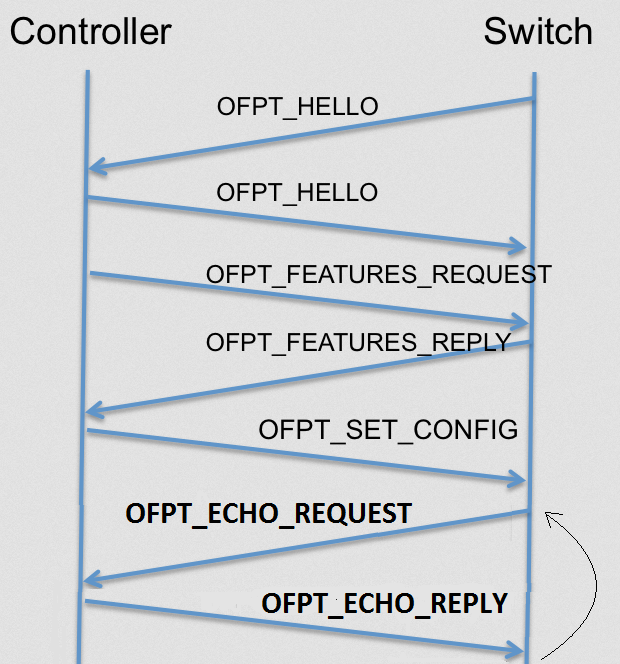
\includegraphics[scale=0.5]{openflow_protocol}
	\centering
	\label{fig:openflow_protocol}
\end{figure}

\begin{figure}[t]
	\caption{Error de comunicación en protocolo de OpenFlow.}
	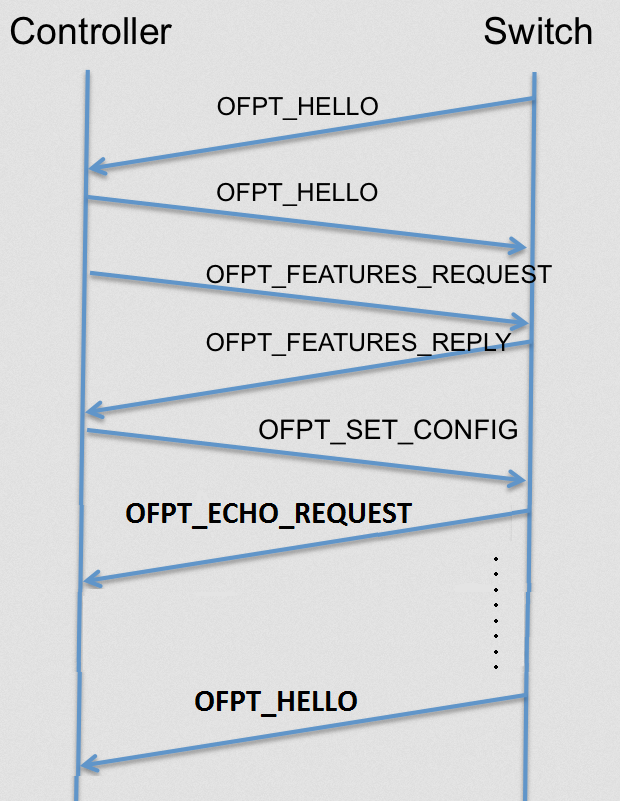
\includegraphics[scale=0.5]{openflow_protocol_error}
	\centering
	\label{fig:openflow_protocol_error}
\end{figure}
De acuerdo al manual de Open vSwitch \cite{ovs-vswitchd-conf}, la variable responsable de este comportamiento es la llamada \textbf{inactivity\_probe}. Se define como el máximo número de mili-segundos que debe esperar el switch antes de enviar un mensaje sonda por inactividad (Echo Request). Si Open vSwitch no se comunica con el controlador por la cantidad especificada de segundos, enviará una sonda, es decir, un mensaje Echo Request. Si la respuesta no es recibida dentro la misma cantidad de mili-segundos adicional, Open vSwitch asume que la conexión se ha finalizado e intenta reconectarse. El valor por defecto para esta variable depende de la implementación, y en el ambiente de trabajo tiene por defecto el número 5000 (5 segundos). Esto quiere decir que si el switch no recibe mensajes del controlador por 10 segundos (5 luego de mandar la sonda) se cerrará la conexión. \\
Lo interesante de esta situación es estudiar por qué el controlador no logra responder a tiempo las sondas de los nodos. Algunas posibles razones son las siguientes:
\begin{itemize}
	\item Congestión en la red de gestión. Es posible que el exceso de nodos genere demasiado tráfico de control, y por ende haya retrasos y/o pérdidas en la red de gestión. Este problema posiblemente estaría presente en un despliegue real de la arquitectura.
	\item Falta de capacidad de cómputo. Dado que este comportamiento se detectó en el entorno virtual y con un número importante de nodos, es posible que el controlador no tenga acceso al poder de cómputo suficiente como para responder a tiempo a todas las sondas. Este sería un problema del entorno virtual, y no sería relevante en una red real.
	\item Incapacidad de Ryu para manejar muchos nodos. En \cite{proyecto-rrap} se menciona que Ryu es un controlador minimalista y académico. Por lo tanto, es posible que no esté diseñado para controlar tantos switches. Si ese fuera el caso, esto sería un obstáculo al desplegar la arquitectura en una red real. 
\end{itemize}
Como solución provisoria, con el propósito de realizar pruebas con las topologias que presentan este problema, se configuró el valor de inactivity\_probe como un número muy alto (45 segundos) de modo de darle al controlador más que suficiente tiempo para responder a las sondas. Sin embargo, esta no es una buena solución ya que en una red real, cuanto más alto esté ese número, más demoraría el controlador en darse cuenta que un switch se desconectó. Se deja para trabajos futuros investigar si esto podría afectar una despliegue real, ya que si lo hace, tendrían que hacerse cambios radicales a la arquitectura.

\subsection{Problema de concurrencia por muchas instancias de OpenVSwitch}
Como se explica en el Proyecto RRAP \cite{proyecto-rrap}, para que las interfaces de red de los nodos funcionen como puertos OpenFlow con dirección IP, no solo se debe crear un puerto en Open vSwitch para cada una, sino que también se debe crear una interfaz virtual con su respectivo puerto. Además, deben crearse flujos para que los paquetes que entran por la interfaz física salgan por su respectiva interfaz virtual, y viceversa.
El siguiente código simplificado muestra como es el proceso de configuración:
\begin{lstlisting}
	ovs-vsctl add-port eth0		#deberia asignar nro de puerto OF 1
	ovs-vsctl add-port eth1		#deberia asignar nro de puerto OF 2
	ovs-vsctl add-port eth2		#deberia asignar nro de puerto OF 3
	ovs-vsctl add-port veth0	#deberia asignar nro de puerto OF 4
	ovs-vsctl add-port veth1	#deberia asignar nro de puerto OF 5
	ovs-vsctl add-port veth2	#deberia asignar nro de puerto OF 6
	
	ovs-ofctl add-flow in_port=1,output:4
	ovs-ofctl add-flow in_port=4,output:1
	ovs-ofctl add-flow in_port=2,output:5
	ovs-ofctl add-flow in_port=5,output:2
	ovs-ofctl add-flow in_port=3,output:6
	ovs-ofctl add-flow in_port=6,output:3
\end{lstlisting}
Cuando se le agrega un puerto, Open vSwitch le asigna automáticamente un número de puerto OpenFlow. La manera en que Open vSwitch hace esa numeración es secuencial, empezando desde 1. Eso quiere decir que, en teoría, si se agregan 3 puertos a Open vSwitch, sus puertos OpenFlow tendrán los números 1, 2 y 3, de acuerdo al orden en que fueron creados. Como se ve en el pseudocódigo, las líneas que agregan los flujos que \enquote{conectan} las interfaces virtuales y físicas asumen que la numeración se hace de esa forma. Está configuración se hace para cada nodo (es decir, para cada instancia de Open vSwitch) y es equivalente a la forma en que se configuran los dispositivos físicos en el prototipo. \\
No se observaron problemas relacionados con esto en topologias chicas de 4 nodos aproximadamente, pero sí en topologias más grandes. Se observó que con más nodos, la numeración de los puertos en Open vSwitch se comportaba de forma impredecible, y no seguía el esquema secuencial que se mencionó anteriormente. Como los flujos que se agregan posteriormente asumen ese determinado orden, eso causa que varias o todas las interfaces del nodo no funcionen. En topologias de entre 10 y 40 nodos ese comportamiento a veces afectaba sólo unos pocos nodos, y en ocasiones no ocurría. Con topologias de 100 nodos aproximadamente, esto ocurría siempre, con más de la mitad de los nodos. Esto llevó a creer que se trataba de un problema de concurrencia por tener muchas instancias de Open vSwitch iniciándose y configurándose al mismo tiempo. \\
Para solucionar este problema se hizo el siguiente cambio:
\begin{lstlisting}
	ovs-vsctl add-port eth0 ofport_request=1
	ovs-vsctl add-port eth1 ofport_request=2
	ovs-vsctl add-port eth2 ofport_request=3
	ovs-vsctl add-port veth0 ofport_request=4
	ovs-vsctl add-port veth1 ofport_request=5
	ovs-vsctl add-port veth2 ofport_request=6
	
	ovs-ofctl add-flow in_port=1,output:4
	ovs-ofctl add-flow in_port=4,output:1
	ovs-ofctl add-flow in_port=2,output:5
	ovs-ofctl add-flow in_port=5,output:2
	ovs-ofctl add-flow in_port=3,output:6
	ovs-ofctl add-flow in_port=6,output:3
\end{lstlisting}
El parámetro opcional \textbf{ofport\_request} permite indicarle a Open vSwitch que número debería asignarle al puerto que se está agregando. Esto soluciona completamente el problema y permite levantar topologias de cualquier tamaño sin problemas. Es importante remarcar que probablemente esto solo afecta al entorno virtual, y no es necesario realizar esta corrección al configurar nodos reales, ya que cada dispositivo ejecuta una única instancia de Open vSwitch y por lo tanto no es probable que se vea este comportamiento. Sin embargo, no se descarta del todo que exista una posibilidad de que esto ocurra, así que se propone el uso de \textbf{ofport\_request} para la configuración de los nodos físicos para eliminar ese riesgo, por más pequeño que sea.

\subsection{Problema de LSDB Sync con muchos nodos}
Explicar problema de read\_all\(\) de python/telnetlib cuando la base es muy grande, y el cambio a read\_very\_eager\(\)
Podría poner que no se encuentra suficiente documentación para explicar el comportamiento, así que se advierte que esto puede afectar una red real tambien y se propone para trabajo futuro.

\subsection{Reducción del MTU}
Explicar que hay que reducir el MTU por 5/10 bytes para iperf

